The fitter and background subtraction procedure, introduced in \Cref{sec:fitting_setup,sec:background_subtraction},
have been thoroughly validated in \Cref{sec:MC_validation} in \MC.
The real challenge, as usual, is ensuring that the conclusions and results observed in \MC generalise correctly to real Belle~II data.
The key concept of a blinded analysis dictates that one must validate the analysis procedure in control samples or regions: collections of data that are abundant, well-understood and provide insight into the behaviour of signal in the detector while being signal free.
In this Section, \FEI validation, 
\piz and $\eta$ veto validation, photon detection efficiency and background modelling is presented.
The combined results from \Crefrange{sec:fei_calibration}{sec:remaining_bb_background_modelling} are shown in \Cref{tab:correction_table}.

\begin{table}[hbtp!]
    \centering
    \caption{\label{tab:correction_table} The corrections for background (and signal in \Cref{sec:validation_efficiency}) efficiency in the hadronic-tagged \BtoXsgamma photon energy spectrum measurement.
    \FEI calibration calculations are discussed in \Cref{sec:fei_calibration}.
    Derivation of correction for the \piz and $\eta$ veto are presented in \Cref{sec:piz_eta_calibration}.
    The photon detection efficiency study is described in \Cref{sec:photon_efficiency}.
    Background modelling corrections are calculated in \Cref{sec:remaining_bb_background_modelling}.
    The \FEI, \piz and \g corrections are averaged values corresponding to the respective \EB bin,
    as the candidate-level information is lost after the \Mbc fit.
    The signal region is highlighted.
    }
    \resizebox{1\textwidth}{!}{
    \begin{tabular}{cccc}
        \hline
        {} \EB, GeV  & FEI calibration & \piz veto correction & \g efficiency correction\\
        \hline
        1.4-1.6  &  \multirow{11}{*}{$0.6630 \pm 0.0229$} & $1.090 \pm 0.050$ & $0.991 \pm 0.023$ \\
        1.6-1.8  &                                        & $1.074 \pm 0.048$ & $0.995 \pm 0.022$ \\
        1.8-2.0  &                                        & $1.064 \pm 0.046$ & $0.996 \pm 0.021$ \\
        2.0-2.1  &                                        & $1.055 \pm 0.046$ & $0.996 \pm 0.021$ \\
        2.1-2.2  &                                        & $1.050 \pm 0.047$ & $0.997 \pm 0.021$ \\
        2.2-2.3  &                                        & $1.046 \pm 0.047$ & $0.997 \pm 0.021$ \\
        2.3-2.4  &                                        & $1.045 \pm 0.047$ & $1.000 \pm 0.020$ \\
        2.4-2.5  &                                        & $1.047 \pm 0.047$ & $1.001 \pm 0.019$ \\
        2.5-2.6  &                                        & $1.050 \pm 0.047$ & $1.001 \pm 0.019$ \\
        2.6-2.7  &                                        & $1.050 \pm 0.046$ & $0.998 \pm 0.019$ \\
        2.7-     &                                        & $1.053 \pm 0.046$ & $0.998 \pm 0.018$ \\
        \hline
        \end{tabular}
}


\end{table}


\subsection{Calibration of the \texorpdfstring{\FEI}{FEI} algorithm}\label{sec:fei_calibration}

The working principle of \FEI has already been discussed in \Cref{sec:tag_reconstruction}.
It combines many classifiers which perform reconstructions of the hadronic decays of \B mesons in various decay chains.
Furthermore, the training of the algorithm happens in \MC.
To ensure that the algorithm appropriately acts on Belle~II data, its performance must be studied or \textit{calibrated}.
The calibration study is performed on data collected by Belle~II, for every simulation campaign, and the work is not part of the original work presented in this thesis.
Full details of the calibration method are presented in Ref.~\cite{Belle-II:2020fst}, but the main details that are relevant to the work of the thesis are summarised here.

The calibration study uses $B\rightarrow X_{u/c} \ell \nu$ decays due to the branching fraction of almost 20~\% and a clean experimental signature, 
where $X_{u/c}$ denotes an inclusive state originating from the $c$ or $u$ quark, similarly to the $X_{s/d}$ notation.
Firstly, in each event, only the highest \FEI probability tag-\B candidate is selected with loose requirements on Fox-Wolfram moments (see \Cref{sec:fox_wolfram_moments}) and $\Delta E$ to ensure adequate \epem\ra\qqbar suppression.
Next, a high energy lepton $p_{\ell}^B>1~\gevc$ is required in each event.
This candidate is required to originate near the interaction point and its identification information from all sub-detectors is required to be consistent with a lepton.

After the selection, a binned likelihood fit for \Mbc is set up, which contains three binned \PDF{s}: signal $B\rightarrow X_{u/c}\ell\nu$ decays, 
secondary or misidentified leptons, and \epem\ra\qqbar events. 
Here, secondary leptons identify leptons coming from the $B$ mesons other than $B\rightarrow X_{u,c}\ell\nu$ decay.
Misidentified leptons are used as a broad term for hadrons whose identification information is consistent with that of either an electron or a muon.
The signal $B\rightarrow X_{u/c}\ell\nu$ \PDF is composed of four sub-\PDF{s}, particularly: $B\rightarrow D\ell\nu$, $B\rightarrow D^*\ell\nu$, $B\rightarrow X_u\ell\nu$ and the rest of  $B\rightarrow X_c\ell\nu$ modes.
The fit is performed separately for the following combinations of tag-\B mesons and lepton:
\begin{itemize}
    \item $B^+$ and $e^-$,
    \item $B^+$ and $\mu^-$,
    \item $B^0$ and $e^-$,
    \item $B^0$ and $\mu^-$.
\end{itemize}
This is shown in \Cref{fig:fei_calib}.
\begin{figure}[hbtp!]
    \centering
    \subcaptionbox{\label{fig:fei_calib_bpluseminus}}{
            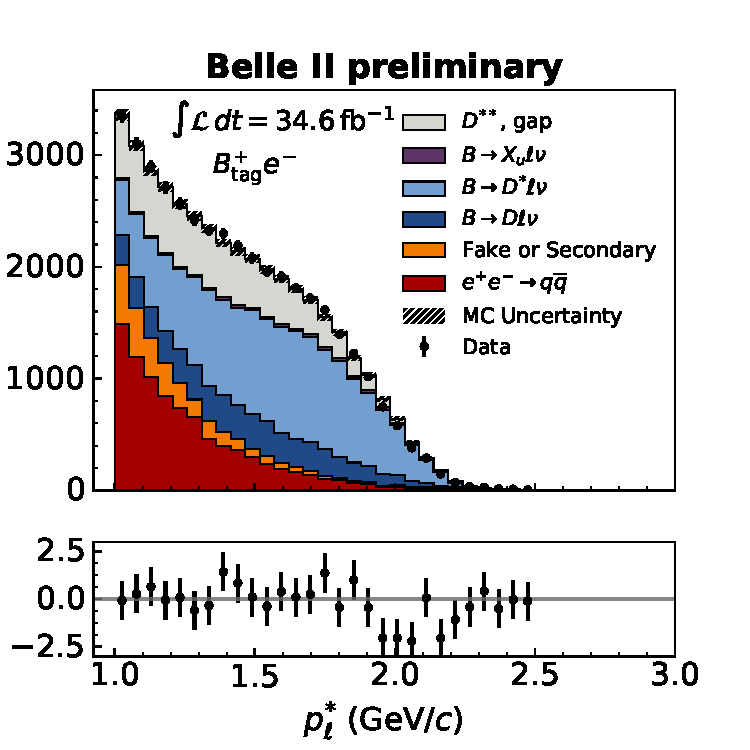
\includegraphics[width=0.45\textwidth]{figures/data_sim_corrections/BpXenu_pl_fit_All_data_postfiterrs.pdf}
    }
    \subcaptionbox{\label{fig:fei_calib_bplusmuminus}}{
            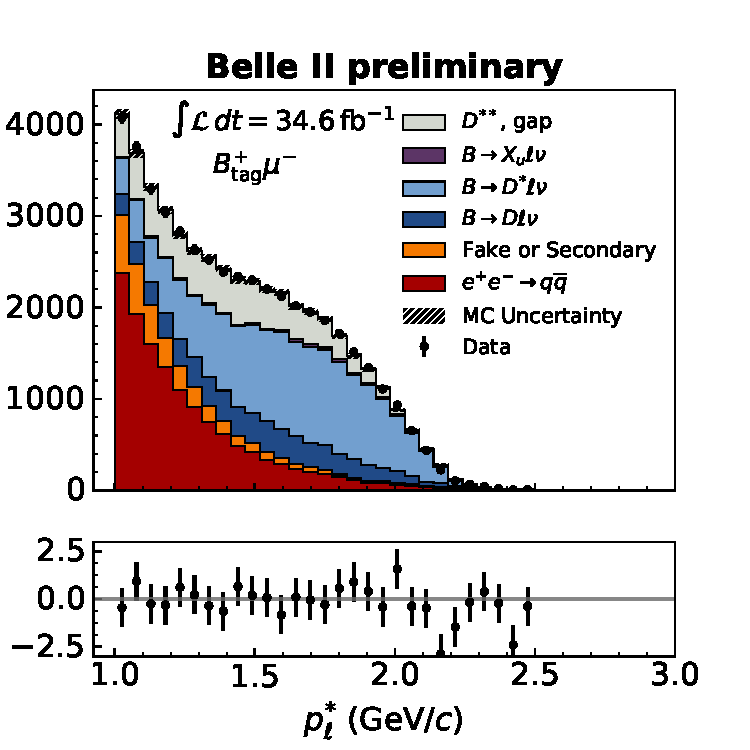
\includegraphics[width=0.45\textwidth]{figures/data_sim_corrections/BpXmunu_pl_fit_All_data_postfiterrs.pdf}
    }
    \subcaptionbox{\label{fig:fei_calib_bzeroeminus}}{
            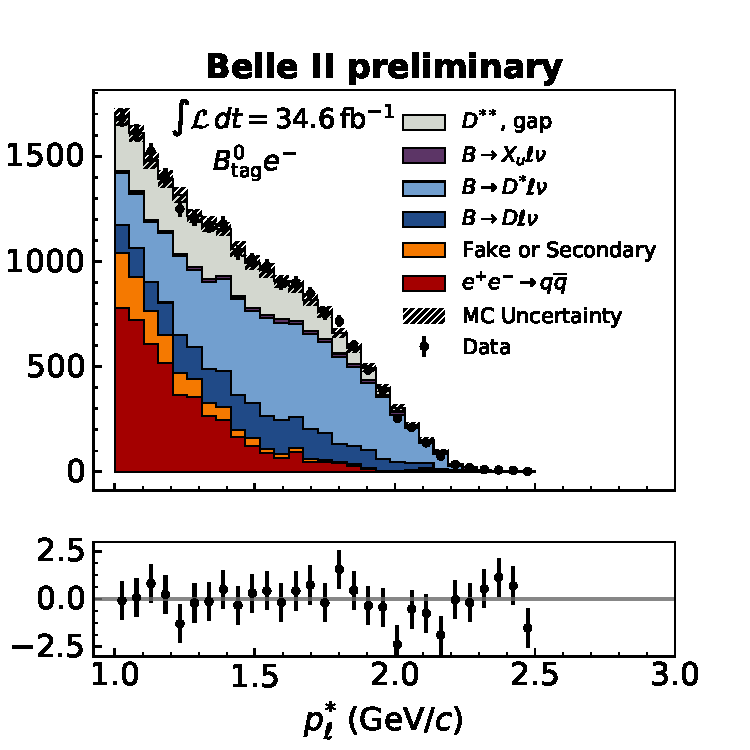
\includegraphics[width=0.45\textwidth]{figures/data_sim_corrections/B0Xenu_pl_fit_All_data_postfiterrs.pdf}
    }
    \subcaptionbox{\label{fig:fei_calib_bzeromuminus}}{
                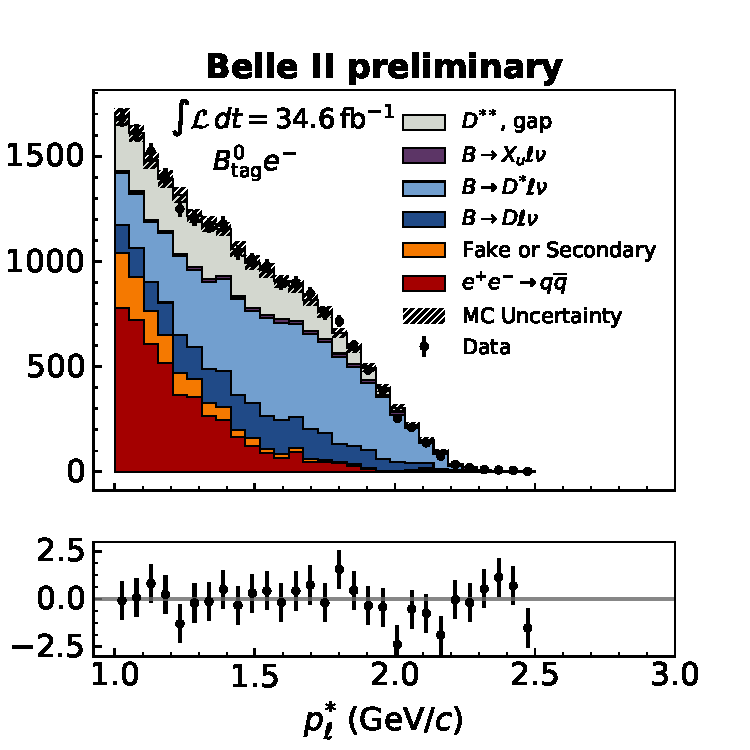
\includegraphics[width=0.45\textwidth]{figures/data_sim_corrections/B0Xenu_pl_fit_All_data_postfiterrs.pdf}
    }
    \caption{\label{fig:fei_calib} Illustration of the fits to \B\to$X_{u/c}\ell\nu$ decays in the \FEI calibration study.
    Results are shown for the combinations of charged and neutral tag-$B$ modes with $e^-$ ((\subref{fig:fei_calib_bpluseminus}) and (\subref{fig:fei_calib_bzeroeminus})) and $\mu^-$ ((\subref{fig:fei_calib_bplusmuminus}) and (\subref{fig:fei_calib_bzeromuminus})).
    Different fit components are shown in the legend and the subpanels contain the pulls of the fit.
    Figures are taken from Ref.~\cite{Belle-II:2020fst}.
    }
\end{figure}

The branching fractions of $B\rightarrow X_{u/c}\ell\nu$ are evaluated from the fitted distributions.
These values are then directly compared with the world average values.
A correction factor, $\mathcal{C}_{\mathrm{FEI}}$, is derived such that the two values become compatible.
The leading evaluated systematic uncertainties come from the imperfect experimental knowledge of the $B\rightarrow X_u\ell\nu$ branching fractions and their form factors, the fit model composition, tracking and particle identification uncertainties.
For the Belle~II simulation campaign used in this analysis, and averaged for both lepton modes, the result is as follows:
\begin{equation}\label{eq:fei_calibration}
    \mathcal{C}_{\mathrm{FEI}}(B^+) = 0.6599 \pm 0.0225; \quad \mathcal{C}_{\mathrm{FEI}}(B^0) = 0.6695 \pm 0.0237,
\end{equation}
where two different calibration factors are presented for \feiBp and \feiBz modes, respectively.
Therefore, for an adequate comparison with Belle~II data, any Belle~II \MC involving the use of \FEI is henceforth scaled appropriately.

\subsection{Calibration of \texorpdfstring{\piz}{pi0} and \texorpdfstring{$\eta$}{eta} suppression tools}\label{sec:piz_eta_calibration}
It was seen in \Cref{sec:selection_vetos} that one of the strongest tools for background suppression in this analysis is the $\piz$ and $\eta$ suppression tool.
Consequentially, any data-simulation discrepancies have a high impact on the final result.
The calibration of the \piz and $\eta$ veto is performed in an independent study and is not part of the original work presented in this thesis 
but the relevant calibration study is discussed in this Section.
Although the calibration analysis only studies \piVeto, it is assumed that the corrections are also valid for \etaVeto selections.
The main concern for the \BtoXsgamma analysis is the primary (signal) photon efficiency: the number of photons that do not originate in light meson decays and get rejected given a certain \piVeto selection.

The calibration study uses $B^+\to \bar{D}^0[\to K^+\pi^-]\pi^+$ and $B^0\to D^-[\to K^+\pi^-\pi^-]\pi^+$ decays, where the square brackets denote a subdecay of the $D$ meson.
The $\pi^+$, originating in the primary $B$ decay, is combined with all other photon candidates in the event in a strategy described in \Cref{sec:selection_vetos} assuming a null-mass hypothesis.
This produces many \piz-like combinations ($\mathit{pseudo}\mathrm{-}\piz$) which yield a \piVeto score with minimal background from real \piz decays.

The reconstruction requires good-quality tracks that originate near the interaction point.
The identification information from Belle~II subdetectors is used to distinguish between pions and kaons.
Because the $\pi^+$ from the primary $B$ decay is combined with other photons, a massless hypothesis is used for calculations of the invariant mass and the helicity angles for the MVA.
After constructing the pseudo-\piz, selections on \piVeto are performed accordingly to those chosen in this analysis.
Therefore, two distributions are created: one with no \piVeto requirement, and a subset distribution with $\piVeto<0.4$.
In both cases, the charged and neutral $B$ channels are combined.

An unbinned \Mbc fit is performed on distributions with and without the \piVeto selections.
The \Mbc is modelled by a Crystal Ball function for signal decays and an ARGUS function for continuum background.
All parameters of Crystal Ball and continuum are unconstrained.
An additional \PDF to model the peaking non-signal \BB components is used.
This \PDF is initialised in \MC as a sum of a Gaussian and an Argus.
The shape parameters and normalisation of the \BB background \PDF are not estimated but kept at the initialised values.
The fits of the data in the case of no \piVeto selection, and a $\piVeto<0.95$ selection are given in \Cref{fig:pivetofit}.
\begin{figure}[hbtp!]
    \centering
    \subcaptionbox{\label{fig:pivetofit_nocut}}{
    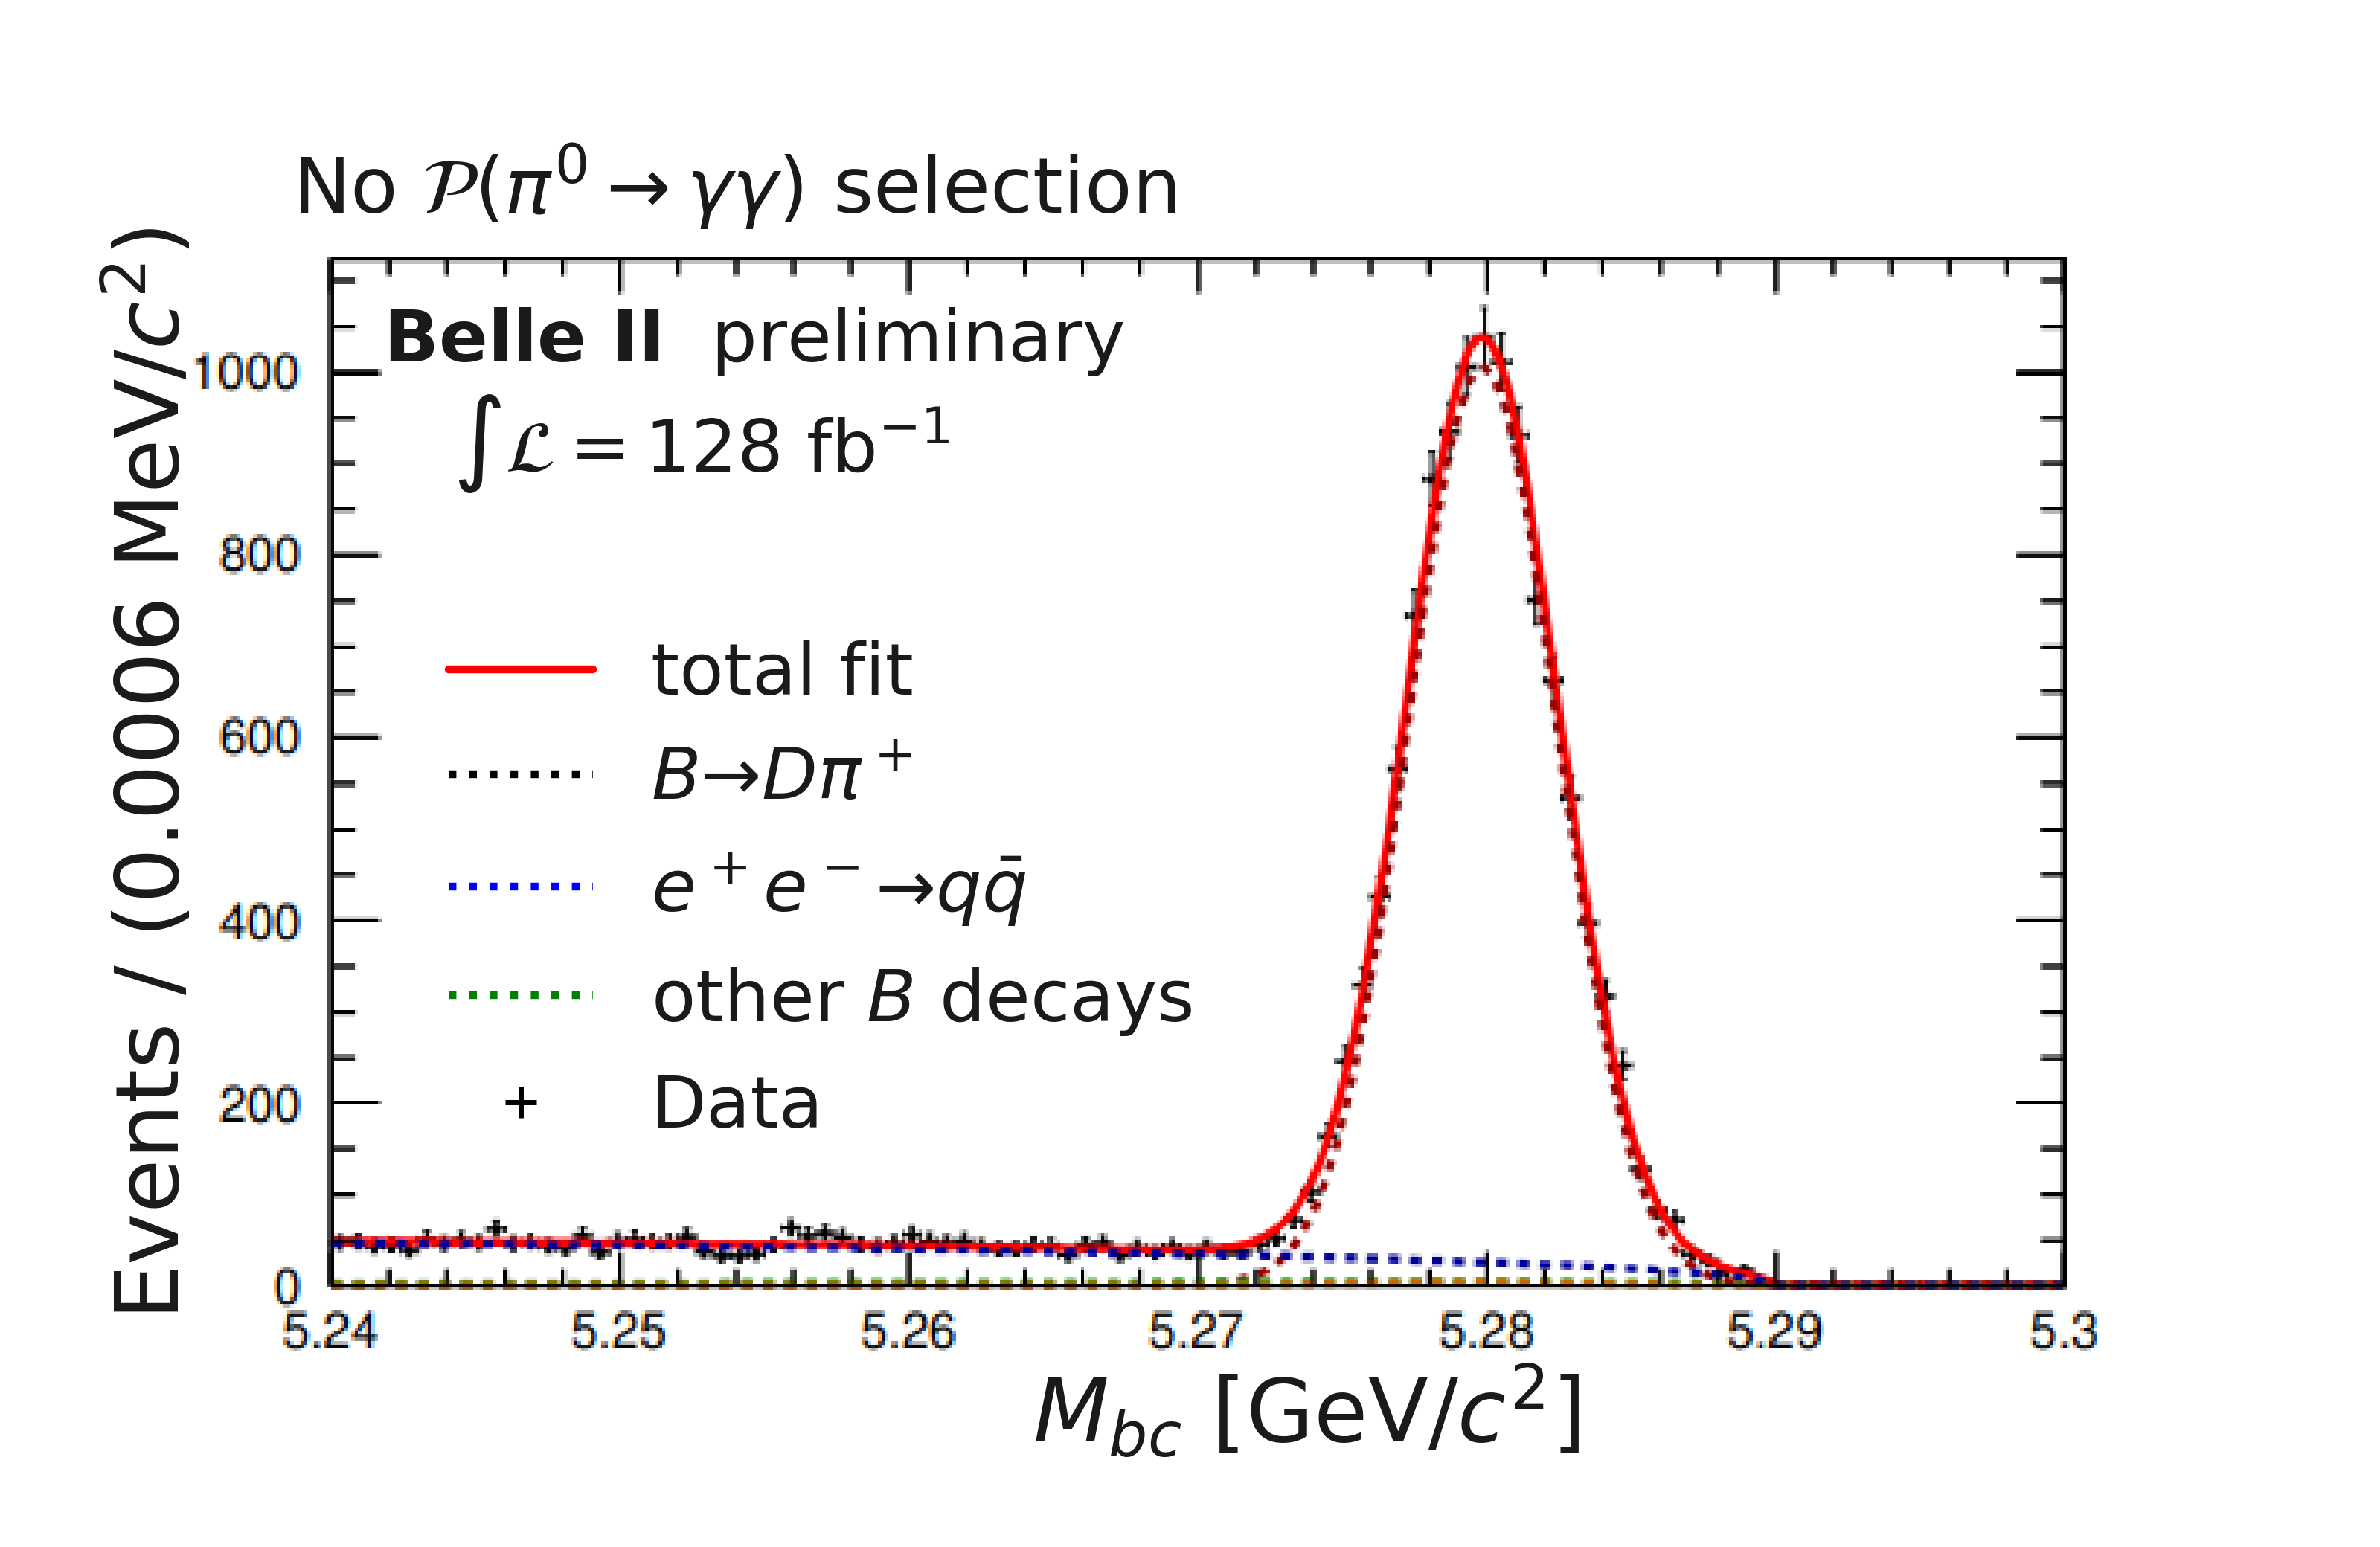
\includegraphics[width=0.45\textwidth]{figures/data_sim_corrections/data_fit_pi0_no_cut.png}
    }
    \subcaptionbox{\label{fig:pivetofit_cut}}{
        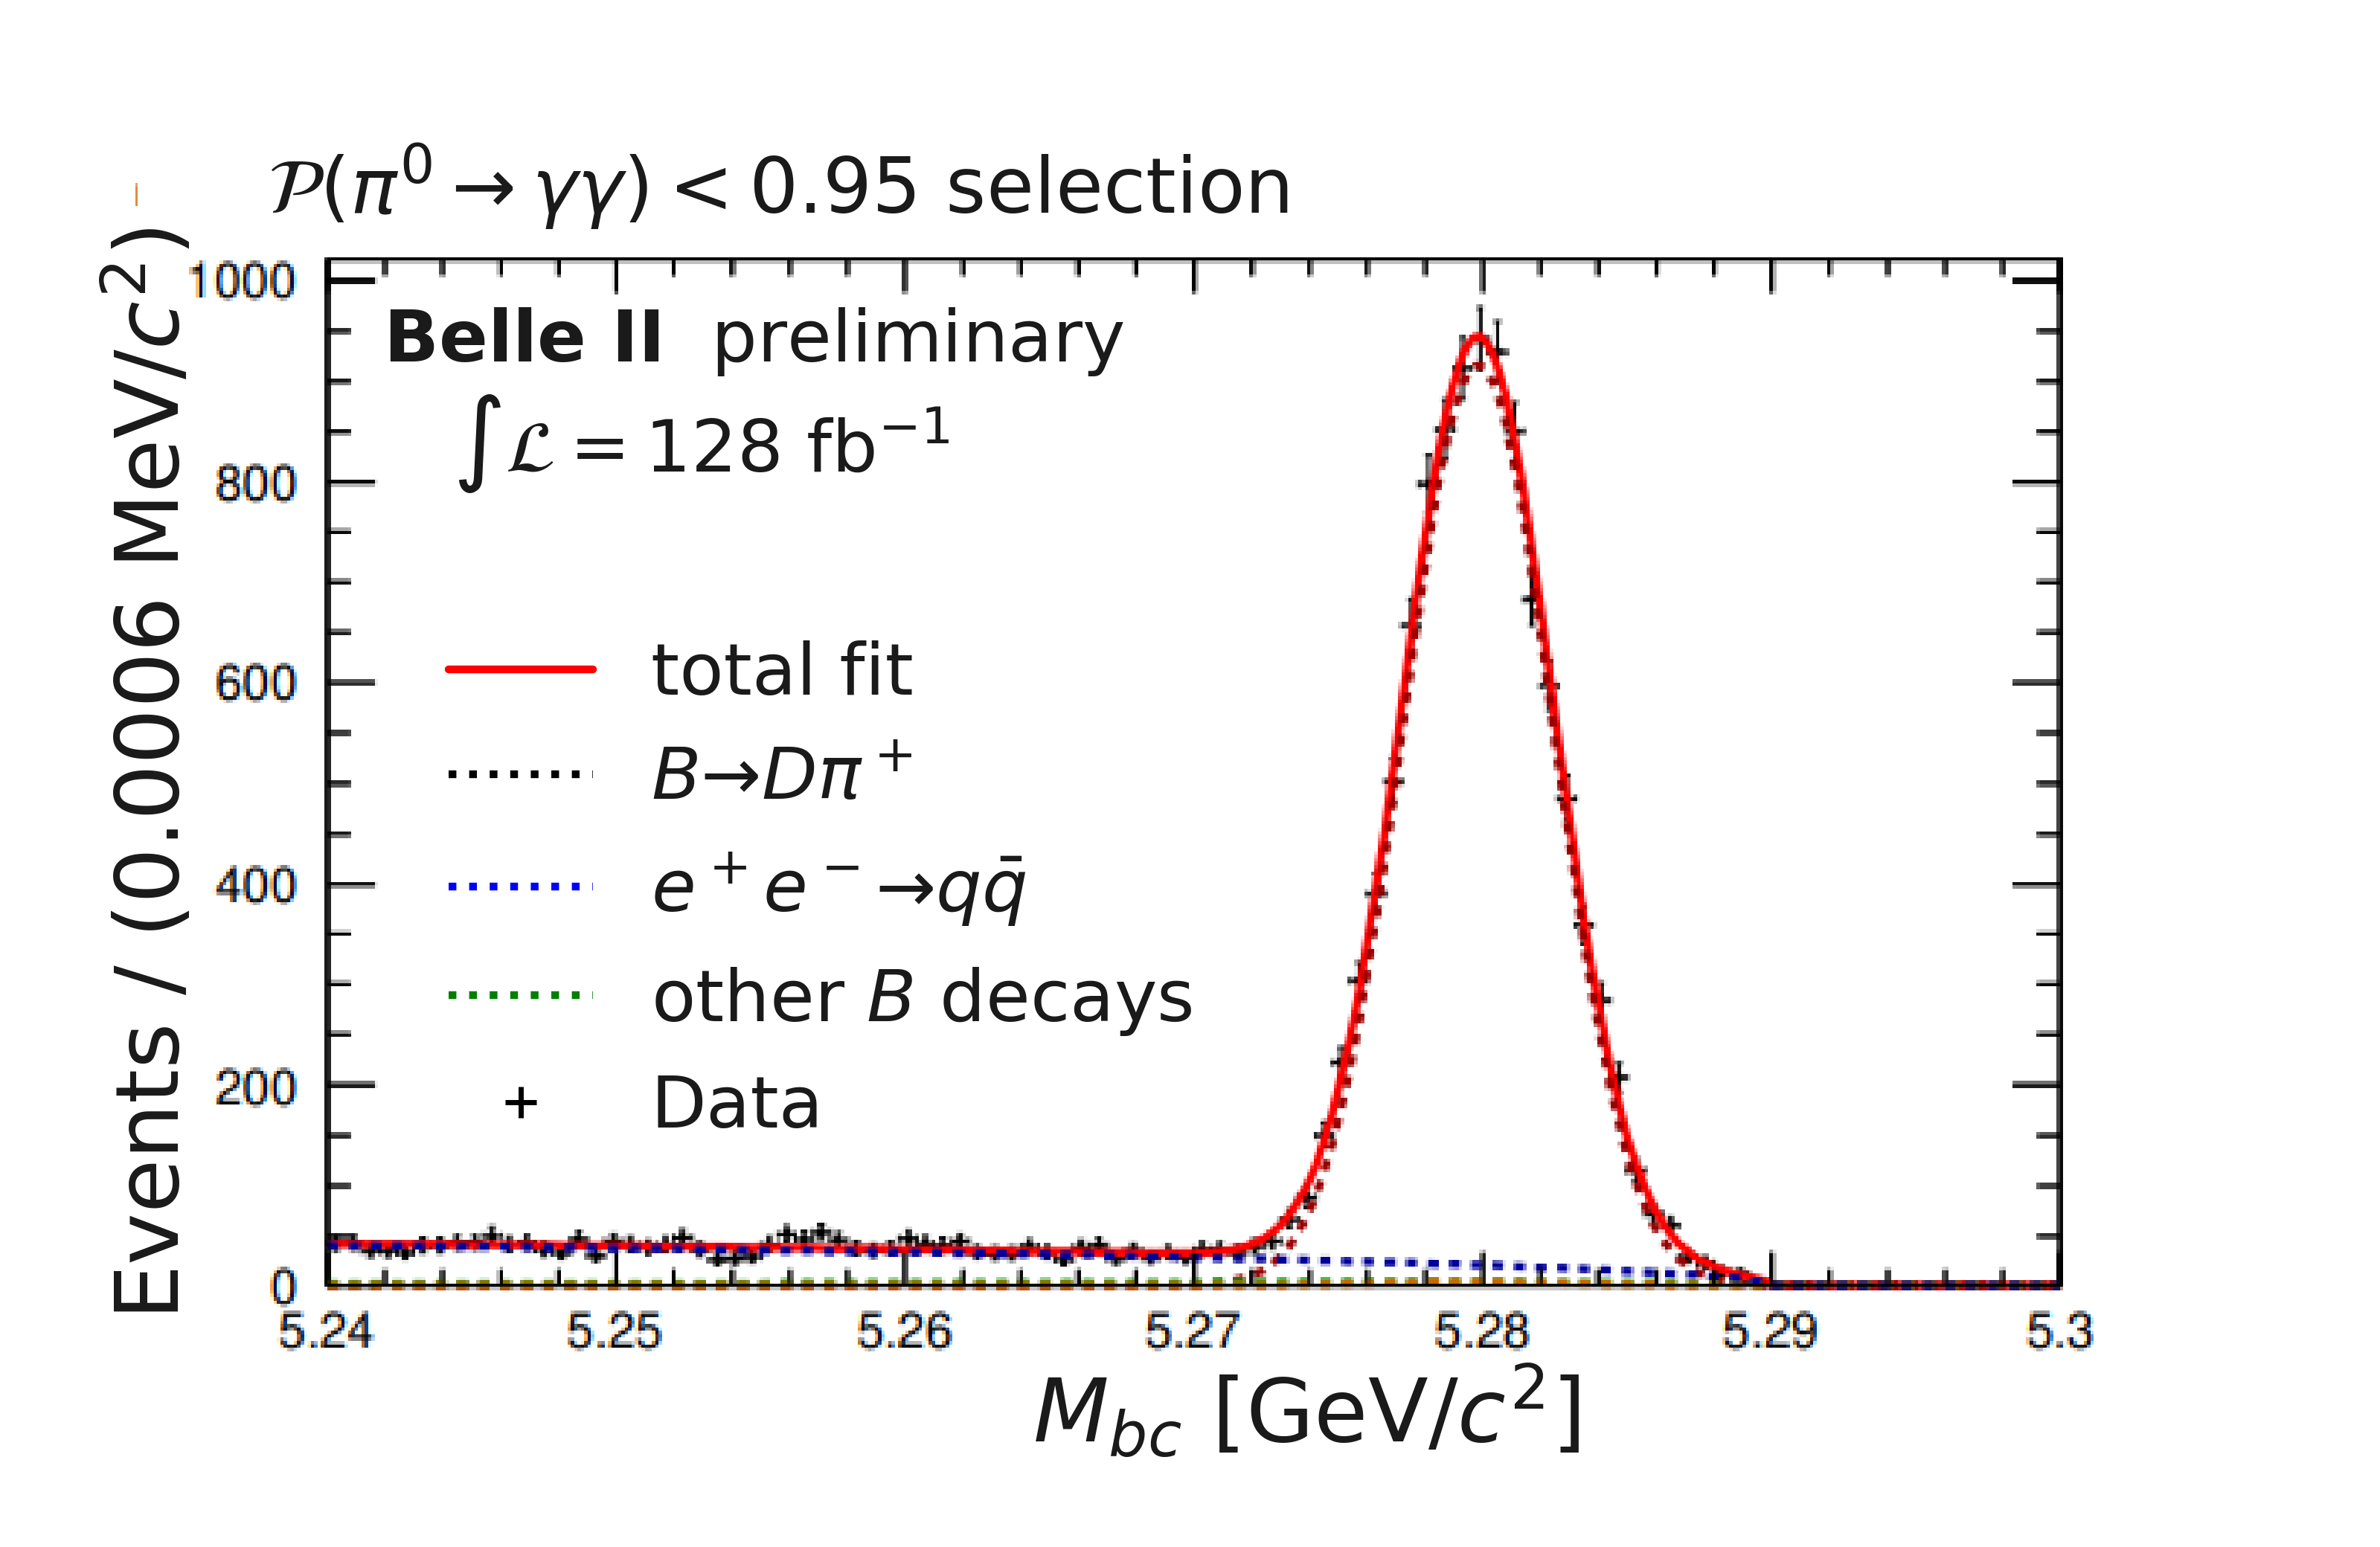
\includegraphics[width=0.45\textwidth]{figures/data_sim_corrections/data_fit_pi0_with_cut.png}
        }
    \caption{\label{fig:pivetofit} The fit estimating the number of $B\to D \pi^+$ events in Belle~II data.
    Different \PDF{s} used in the fit are shown in the legend and explained in the text.
    The fit is performed on a sample without (\subref{fig:pivetofit_nocut}) and with (\subref{fig:pivetofit_cut}) the \piVeto selection applied.
    The extracted values from \MC and data are then combined to calculate \piVeto correction factors (see \Cref{eq:piveto_correction}).
    These Figures are produced by a Belle~II internal study of the \piz veto and are not part of the original work in this thesis.
    Only the labels and legends have been adapted.    
    }
\end{figure}

The fit extracts the counts of $B\to D\pi^+$ events, $N_{B\to D\pi^+}$, as the normalisation parameter of the Crystal Ball.
An efficiency, $\varepsilon\equiv N_{B\to D\pi^+}/N^{\piVeto<0.4}_{B\to D\pi^+}$ is defined, which corresponds to the primary photon efficiency.
If the fit is performed in \MC and data, an efficiency ratio can be used as a correction factor:
\begin{equation}\label{eq:piveto_correction}
    R_{\piVeto} = \frac{N_{B\to D\pi^+}/N^{\piVeto<0.4}_{B\to D\pi^+}|_{\mathrm{data}}}{N_{B\to D\pi^+}/N^{\piVeto<0.4}_{B\to D\pi^+}|_{\mathrm{MC}}}.
\end{equation}
The corrections are calculated in $200~\mev$ intervals of the laboratory frame energy of the primary $\pi^+$.
Results for corresponding to selection chosen in this analysis are given in \Cref{fig:piveto_corrections}.
The internal Belle~II study providing these corrections was only performed in the range of 1.8 to 3.0~\gev in the laboratory frame energy of the primary $\pi^+$.
A linear extrapolation is performed to estimate the values outside the range.
It is observed that the linear extrapolation is consistent, within errors, with the corrections in $1.8-3.0~\gev$.
Therefore, a correction factor of $1.10\pm0.05$ is chosen for events outside the range covered by the calibration study.
This value is consistent with the correction factors in other \Egamma bins.
\begin{figure}[hbtp!]
    \centering
    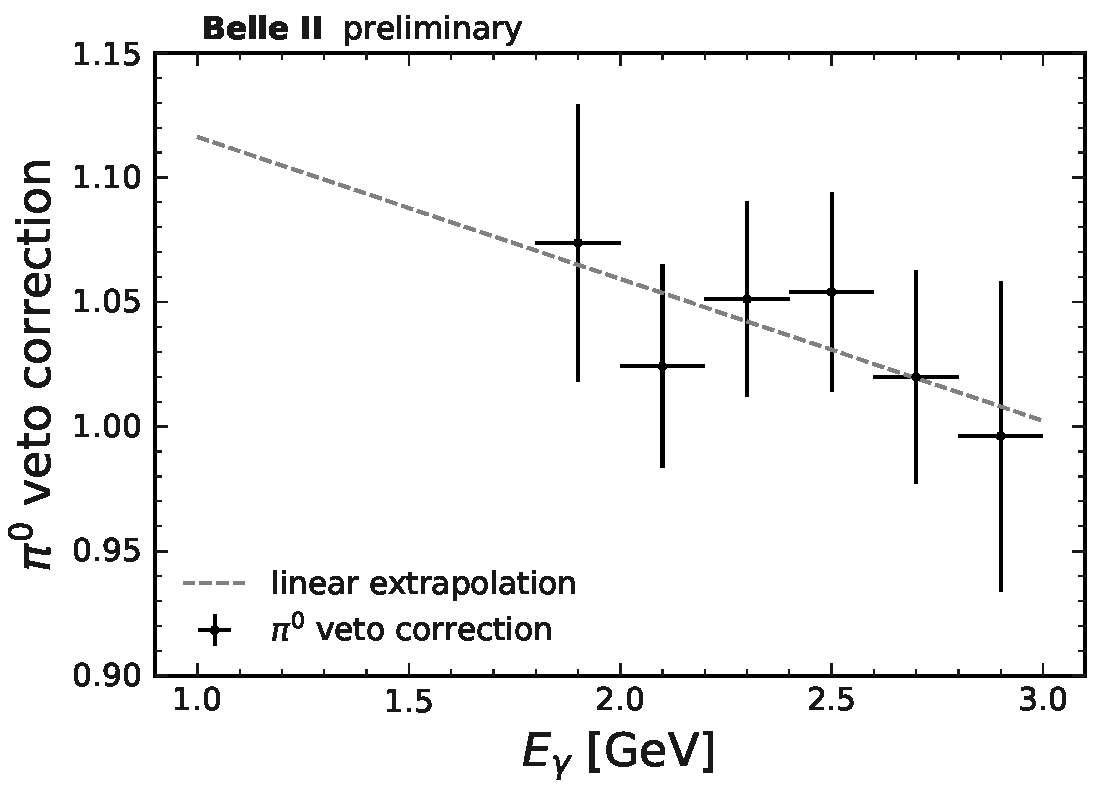
\includegraphics[width=0.45\textwidth]{figures/data_sim_corrections/pi0veto_corrections.pdf}
    \caption{\label{fig:piveto_corrections} The corrections $R_{\piVeto}$ for the $\piVeto<0.4$ selection used in this analysis.
    The results cover $1.8-3.0~\gev$ energies in the laboratory frame, $\Egamma$.
    Because the laboratory frame energies cannot be trivially transformed to the $B$ meson rest frame energies, a linear extrapolation to lower energies is performed as identified by the dashed line.
    }
\end{figure}

\subsection{Belle~II calorimeter photon detection efficiency}\label{sec:photon_efficiency}

One of the main necessities of a measurement involving photons in the final state, is, of course, a precise and accurate simulation of the \ECL.
Although it is designed with precision and resolution suitable for flavour physics studies, 
exact data-simulation differences have to be evaluated.
A Belle~II calorimeter photon detection efficiency study has been performed.
The initial setup of the analysis has been prepared by Dr.~Natalia Kovalchuk and Prof.~Dr.~Torben Ferber. 
However, as part of the original work presented in this thesis, the analysis was updated and reworked for later versions of Belle~II data. 
It also supplemented the initial studies with a full systematic uncertainty evaluation.
While it is a critical study for the \BtoXsgamma analysis, the results are also routinely used in other analyses that utilise photons in their final states.
The study is summarised in a Belle~II public note \cite{Henrikas:2604}.
Here, the main measurement concepts and the results relevant to the measurement of \BtoXsgamma are presented.

To measure the photon detection efficiency, one must first have the knowledge that a photon has been created in an event and then search for it within the calorimeter.
In this efficiency study, $\epem\ra\mumu$ scattering events are employed.
In particular, collision events where a high energy photon is radiated in the initial state are sought.
The concept of the efficiency measurement is sketched in \Cref{fig:photon_efficiency_measurement}.
\begin{figure}[hbtp!]
    \centering
    \subcaptionbox{\label{fig:eemumugamma_feynman}}{
    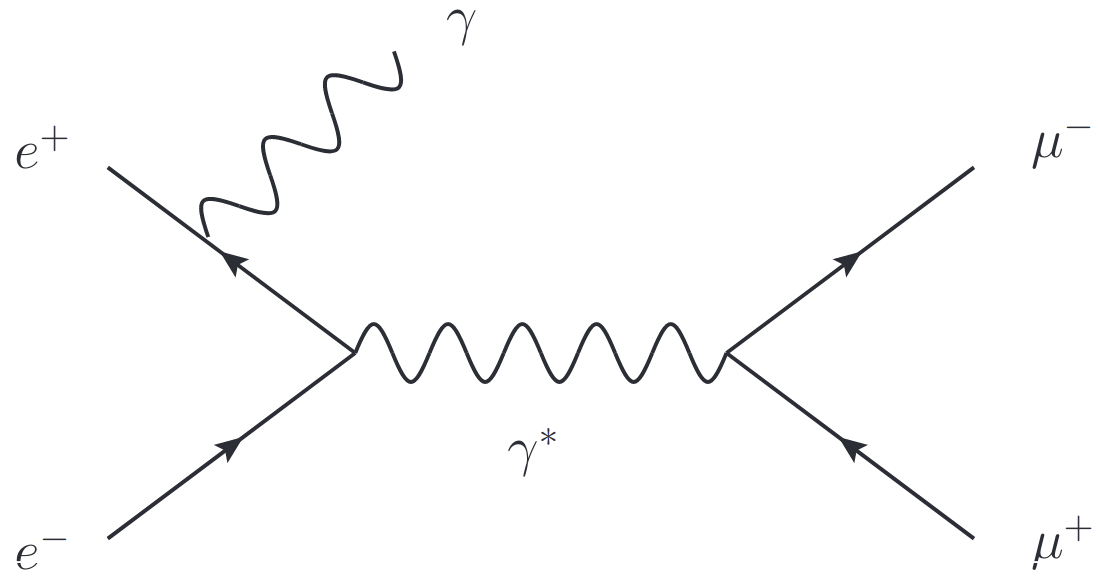
\includegraphics[width=0.4\textwidth]{figures/data_sim_corrections/eemumugamma.png}
    }
    \subcaptionbox{\label{fig:measurement_principle_gammaeff}}{
        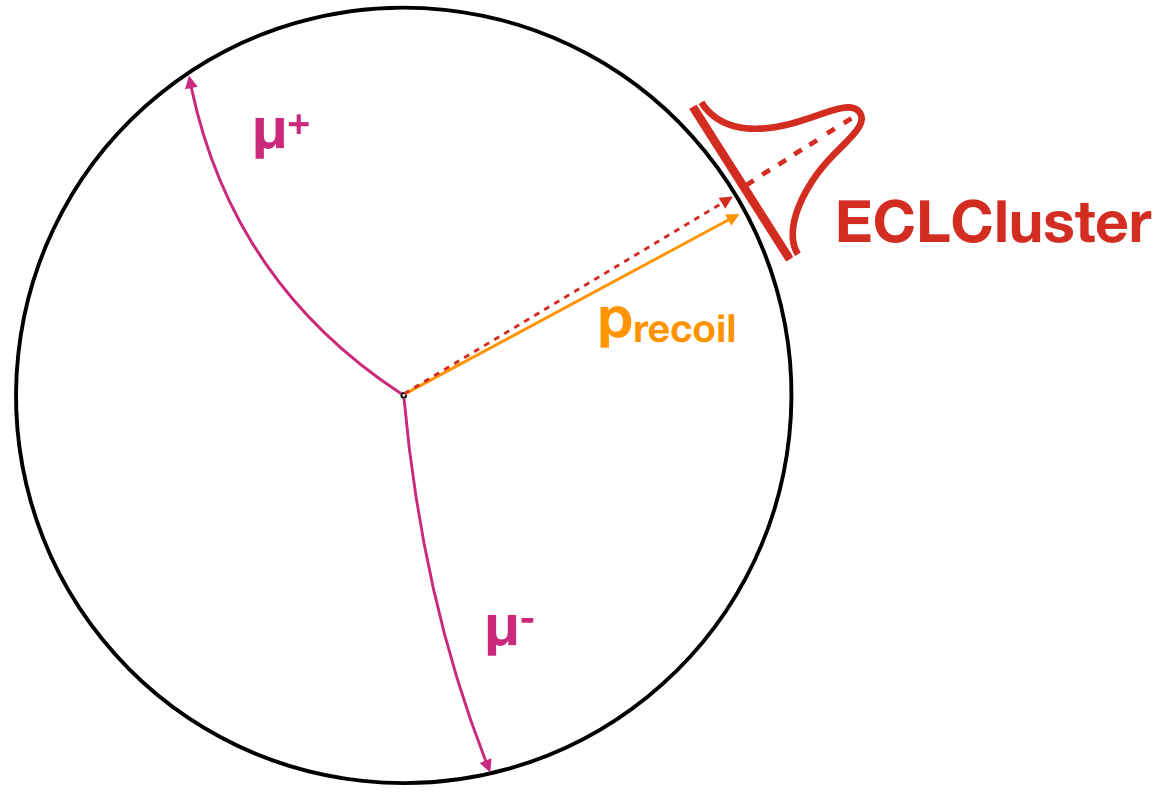
\includegraphics[width=0.4\textwidth]{figures/data_sim_corrections/measurement_principle.png}
        }
    \caption{\label{fig:photon_efficiency_measurement} The main concepts of the measurement of the Belle~II photon detection efficiency.
    The Feynman diagram of the $\epem\ra\mumu$ events, where a photon is radiated in the initial collision state, is shown in (\subref{fig:eemumugamma_feynman}).
    Due to the radiated photon, the resulting dimuon system will have a missing momentum with respect to the usual collision energy $\sqrt{s}\approx10.58~\gev$.
    The direction of the missing momentum can be extrapolated to search for photon clusters in the calorimeter, as sketched in (\subref{fig:measurement_principle_gammaeff}).
    }
\end{figure}

The main goal is to reconstruct two muon tracks in each event and evaluate their total momentum and energy.
If a high energy photon (further called initial-state radiation or \ISR) is created before the collision, the energy of the dimuon system has a certain degree of missing-momentum whose direction coincides with that of the emitted photon.
This missing momentum direction is called \textit{recoil} and is characterised by the magnitude (equivalent to the photon energy), polar angle and azimuthal angle.
Therefore, by selecting events where such recoil is present, one looks for photon clusters corresponding to the angle and the energy within the calorimeter.
This gives a photon detection efficiency estimate through a simple event counting relation:
\begin{equation}\label{eq:photon_efficiency}
    \varepsilon_{\gamma}(|\vec{p}_{\mathrm{recoil}}|, \theta_{\mathrm{recoil}}, \phi_{\mathrm{recoil}}) = \frac{N(\mathrm{photon~found}~\cup~\mathrm{recoil~found})}{N(\mathrm{recoil~found})},
\end{equation}
which can be evaluated as a function of missing momentum with a magnitude $|\vec{p}_{\mathrm{recoil}}|$ and corresponding angles $\theta$ and $\phi$.

Many background processes degrade the efficiency by producing events with sufficient recoil momentum.
A notable example is the $\epem\ra\tautau$ events which may produce two muons and four neutrinos through subsequent $\tau$ decays.
The presence of neutrinos creates a missing momentum which mimics the recoil that originates from an \ISR photon.
Furthermore, tracking inefficiencies can lead to an incorrect measurement of the direction or magnitude of the recoil vector.
Finally, two or more \ISR photons per event further complicate the photon finding procedure, resulting in an overall drop in efficiency.
Therefore, \Cref{eq:photon_efficiency} is more correctly referred to as \textit{photon finding efficiency}, rather than photon detection efficiency.

The photon finding inefficiency effects are suppressed to a certain degree through a double ratio measurement:
\begin{equation}\label{eq:photon_data_mc}
    R_{\gamma} = \frac{\varepsilon_{\gamma}^{\mathrm{DATA}}}{\varepsilon_{\gamma}^{\mathrm{MC}}},
\end{equation}
where $\varepsilon_{\gamma}$ are respective values of photon finding efficiency calculated in data or simulation, based on \Cref{eq:photon_efficiency}.
The double ratio, $R_{\gamma}$, is considered the photon detection efficiency data-to-simulation ratio in this analysis.

First, tracks consistent with $\epem\ra\mumu$ processes are selected by requiring each event to have exactly two charged tracks that:
\begin{itemize}
    \item have a high-momentum requirement $p>1~\gevc$;
    \item are consistent to have originated from the interaction point;
    \item act as a minimum ionising particle in the \ECL: leave energy deposits smaller than 300~\mev and less than 80\% of the total momentum.
\end{itemize}
The two muon tracks passing these requirements are used to evaluate the missing energy and momentum of the event, requiring the recoil magnitude $p_{\mathrm{recoil}}>0.2~\gevc$.
Backgrounds from various $\epem\ra\mathrm{hadrons}$ or $\epem\ra\tautau$ are strongly suppressed by the mass associated with the missing momentum requirement,
$m^2_{\mathrm{Recoil}}<2~\gev/c^4$.
This requirement ensures that the particle associated with the missing momentum is consistent with a photon.
Generally, this does not have to be true for non $\epem\ra\mumu(\gamma)$ events where more than two tracks are present.
Additional checks, such as sufficient isolation of the muon tracks and the recoil are required to ensure adequate separation between their energy deposits in the \ECL.
If all the aforementioned requirements are passed, an event is considered to have a \textit{recoil found}.
The distributions for events with a recoil found are shown in \Cref{fig:selected_photon_data_mc}.

The photon candidates are selected by requiring them to have a centre-of-mass energy of at least $75~\mev$ and a timing of the associated cluster at $\pm200~\ns$.
These requirements were optimised to reduce the impact of beam background photons.
No tighter selections on photons or their reconstruction quality are made to ensure that no bias is introduced in the detection efficiency.

The recoil candidates are matched to photon clusters in the \ECL via two matching requirements:
\begin{itemize}
    \item Photons have to be within 0.3~\rad cone around the recoil direction;
    \item The cluster energy to recoil momentum ratio must satisfy $1.2>E_{\gamma}/\pRecoil>0.5$.
\end{itemize}
If both requirements are fulfilled the event is considered to have a \textit{photon found}.
The distribution of events where the recoil is successfully matched to a photon is given in \Cref{fig:matched_photon_data_mc}.
\begin{figure}[hbtp!]
    \centering
    \subcaptionbox{\label{fig:selected_photon_data_mc}}{
    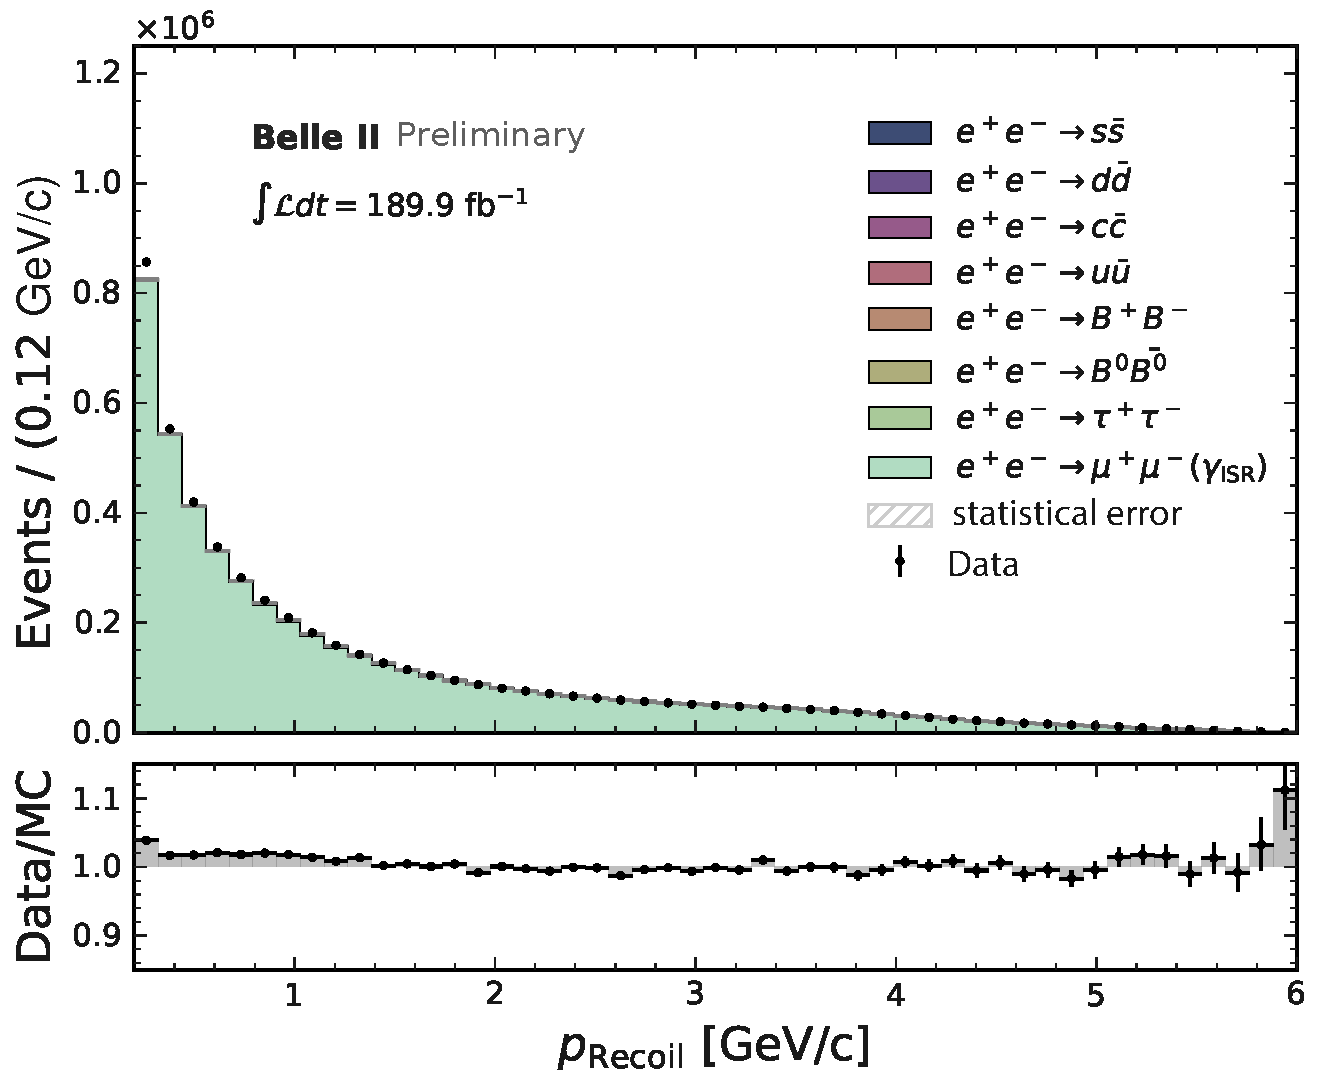
\includegraphics[width=0.45\textwidth]{figures/data_sim_corrections/pyth_data_normalisation_to_mc_comparison_pRecoil_selected_repaired.pdf}
    }
    \subcaptionbox{\label{fig:matched_photon_data_mc}}{
        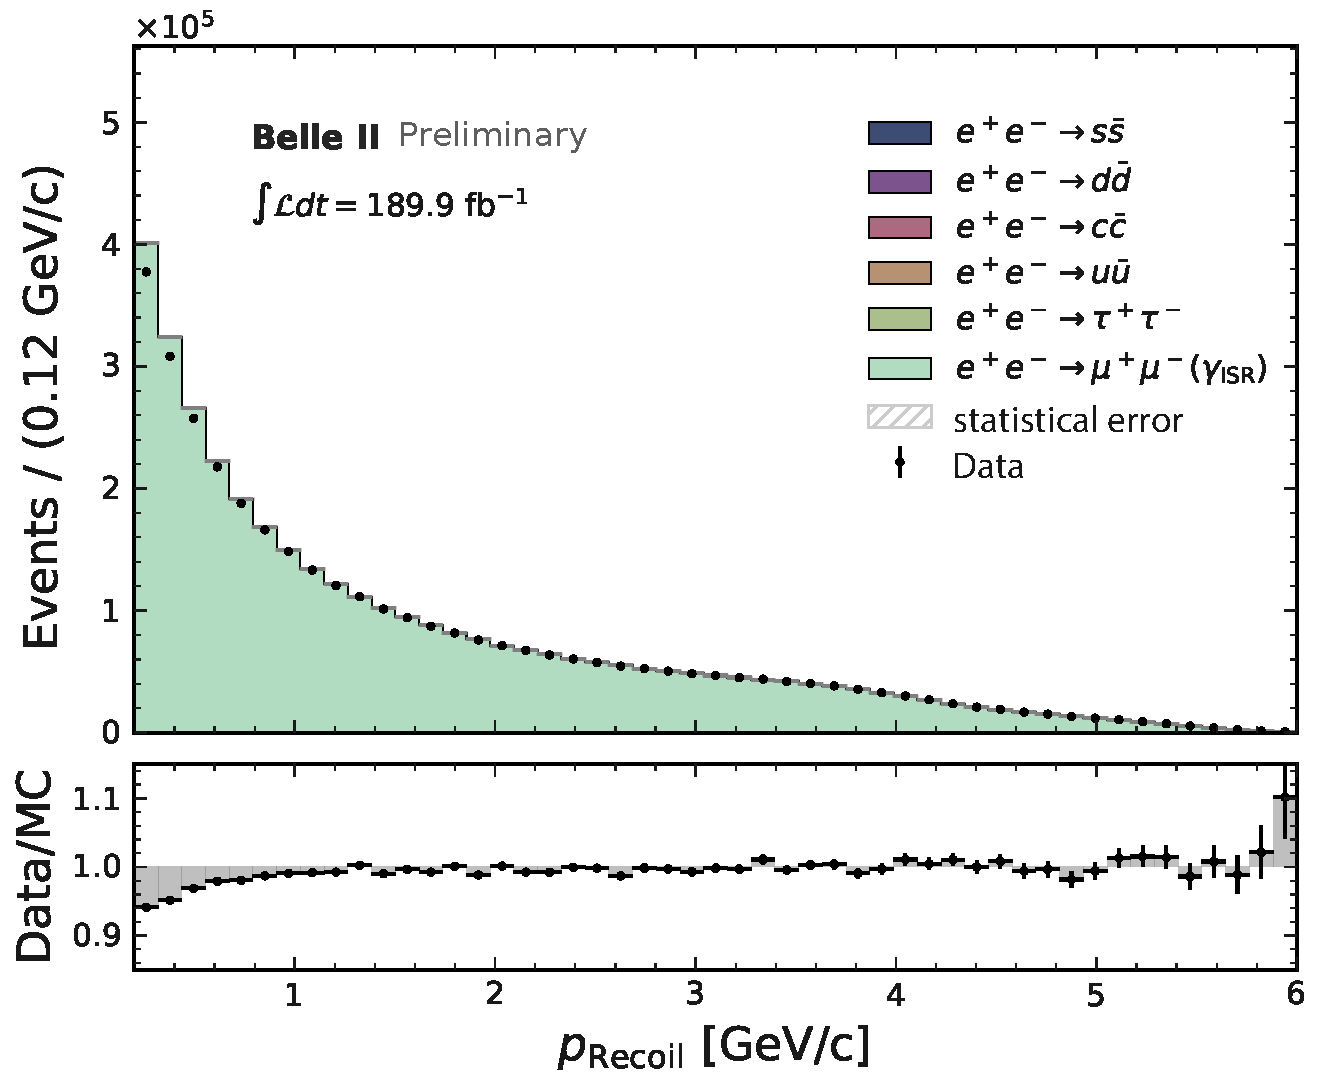
\includegraphics[width=0.45\textwidth]{figures/data_sim_corrections/pyth_data_normalisation_to_mc_comparison_pRecoil_matched_repaired.pdf}
    }
    \caption{\label{fig:normalisation_data_mc} Distribution of $\epem\ra\mumu$ events with a photon radiated in the initial interaction state, as a function of the magnitude of the missing momentum of the dimuon system.
    Events where a missing momentum has been found are shown in (\subref{fig:selected_photon_data_mc}).
    Events where a missing momentum has been found and it was consistent with a photon in the calorimeter, as discussed in the text, are shown in (\subref{fig:matched_photon_data_mc}).
    Various sources of background events are also included, and they can be seen to be at a low level.
    Overall, the signal and background events describe data accurately.
    The subpanels show the data-to-simulation ratio.
    These Figures contain only statistical uncertainties.
    They show the results for the data sets of a size equivalent to the ones used in this analysis.
    }
\end{figure}

The events represented in \Cref{fig:selected_photon_data_mc} reflect the content of the numerator of \Cref{eq:photon_efficiency}, whereas \Cref{fig:matched_photon_data_mc} -- that of the denominator.
The finding efficiencies and their ratio in data and \MC are calculated.
The expected backgrounds, evaluated in \MC, are subtracted from the data distributions.
The results are shown in \Cref{fig:data_mc_photon_eff}.
The data-to-simulation ratio is generally high and approximately equal to unity for photons above 1~\gev.
A drop-off for low energy photons (low \pRecoil) is attributed to the presence of soft \ISR photons in the event which affect the direction of the recoil.
This effect becomes larger with the lower photon energy, where the impact of a second \ISR photon grows.
\begin{figure}[hbtp!]
    \centering
    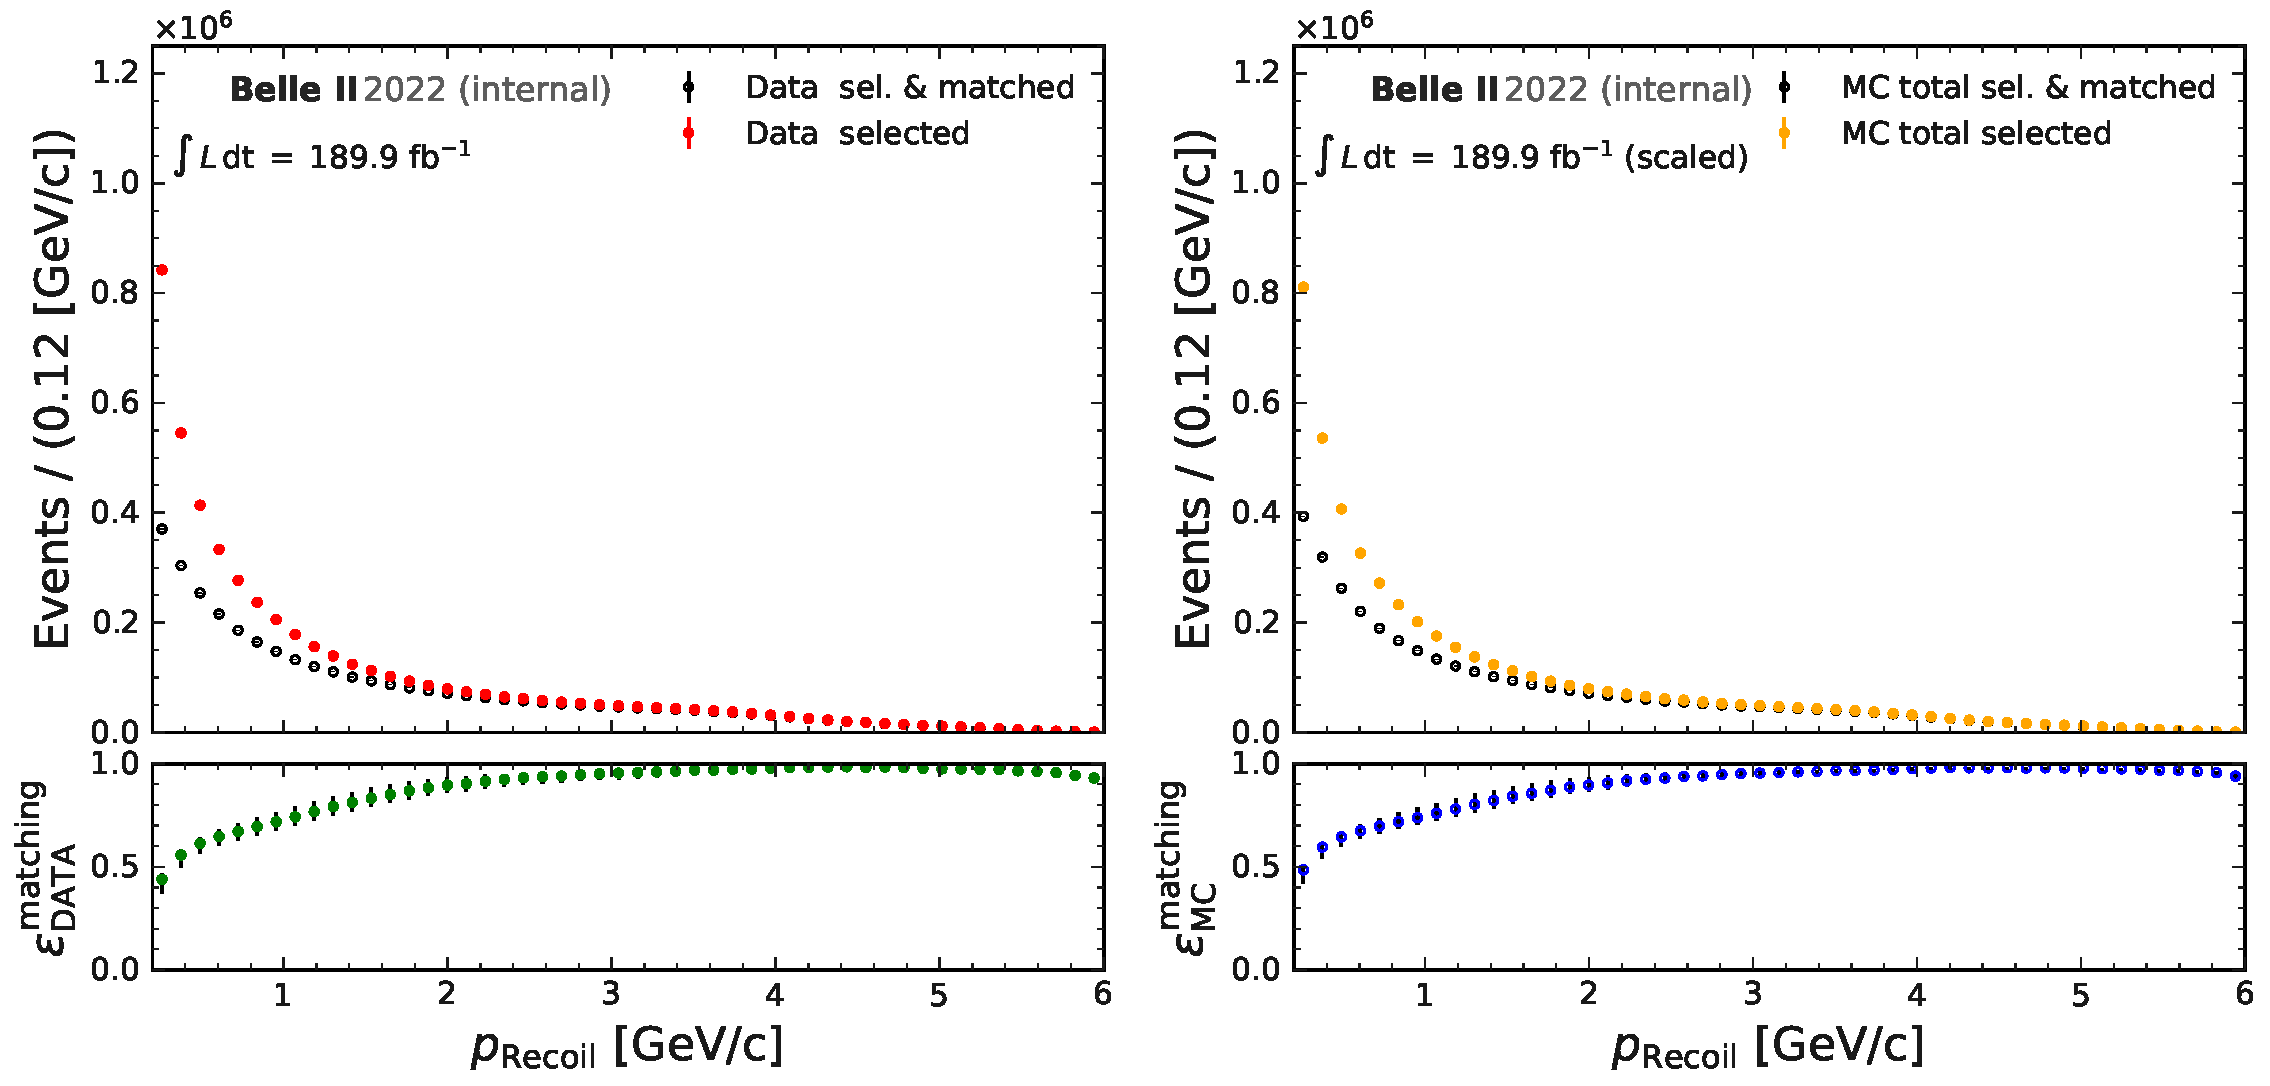
\includegraphics[width=0.45\textwidth]{figures/data_sim_corrections/pyth_data_mc_agreement_pRecoil.pdf}
    \caption{\label{fig:data_mc_photon_eff} The photon finding efficiency as a function of the missing momentum of the dimuon system, \pRecoil.
    The subpanel shows the ratio of data and simulation finding efficiencies, as per \Cref{eq:photon_data_mc}.
    The Figures include systematic uncertainties, which are correlated between data and \MC.
    They show the results for the data sets of a size equivalent to the ones used in this analysis.
    }
\end{figure}

The systematic uncertainties are also calculated.
Most of the selections are tightened and loosened to evaluate the dependence of efficiency on selection requirements.
The maximum shifts in the central value are assigned as systematic uncertainties.
A full shift to the central value without the remaining background subtraction in data is also added as a systematic uncertainty.
The largest systematic uncertainties arise from the leftover background modelling, $m^2_{\mathrm{Recoil}}$ selection variations and muon calorimeter energy deposit variation requirements.
In total they are at $\order(1\%)$ level.

Equivalent distributions to \Cref{fig:normalisation_data_mc} as 3-D functions of \pRecoil, \pRecoilPhi and \pRecoilTheta are produced and 3-D efficiency maps are calculated.
Based on the detected photon direction and energy, appropriate corrections are applied.
In the \BtoXsgamma analysis, the event-level information is lost after performing the \Mbc fit and subtracting the remaining \BB background.
Therefore, the average corrections are evaluated with the \BtoXsgamma hybrid-signal model based on the \EB spectrum binning.
These values are provided in \Cref{tab:correction_table}.

\subsection{Modelling of remaining-\texorpdfstring{\BB}{BB} background processes}\label{sec:remaining_bb_background_modelling}

While the results of previous Sections correct for the procedures used in the removal of photon and tag-side backgrounds, they do not account for any discrepancies that may be introduced when generating the \MC.
Although a full study of all possible background modes that may contribute to the leftover \BB background and their description in the Belle~II simulation is outside of the scope of this work, 
the adequacy of background simulation is studied for the analysis presented here.
In general, the Belle~II \MC is validated and known to produce an accurate and precise simulation of most processes that are common to $B$-factories.
However, our knowledge of the nature and the Standard Model is constantly improving, therefore, the branching fractions or other parameters used in the generation of the generic \BB simulation may not be updated in time as the simulation campaigns happen roughly yearly.
The goal of this study is to check that the generated branching fractions of the main backgrounds that contribute to \BtoXsgamma match those reported by Ref.~\cite{Workman:2022ynf}.

First, only events contributing to good tag-\B mesons based on studies in \Cref{sec:good_tag_definition} are selected.
In each \EB interval, all (non-\BtoXsgamma) $B$ decay modes that produce high-energy photon candidates are selected.
The modes are ranked by their relative abundance within that \EB interval.
Particularly in the low-\EB region, there are hundreds of different $B$ meson decay channels that can contribute to the background.
Pragmatically, only background $B$ decays that contribute at least 1\% to the background in at least one \EB interval are further considered.
These requirements encompass 53 \Bp modes and 39 \Bz decay modes. 
They are listed in \Cref{tab:leftover_bp} and \Cref{tab:leftover_bz}, respectively.
These Tables also contain their relative abundances in every given bin.
As hundreds of $B$ decay modes contribute at $\order(<1\%)$ relative abundance, these requirements may not cover all background modes. 
However, it is assumed that the corrections for non-dominant background modes should on average be unity, as large branching fraction differences in Belle~II simulation are not expected.

The main sources of background photons come from various $B\to D$ transitions, where photons originate from either subsequent $D$ decays or the accompanying particle, e.g. $B\to D\rho$.
Semileptonic $B$ decays are also a major source of background.
In general, $B\to D$ transitions are largely dominating up to $2.2-2.3~\gev$.
At higher \EB, other types of decays become prominent, but more sporadically and without clearly dominating modes.
In particular, various rare $B$ decays, such as $B\to K$, $B\to\pi$ and $B\to\eta$ transitions become more prominent.

The selected background $B$ decay modes have their branching fraction in the Belle~II simulation files compared with that reported by Ref.~\cite{Workman:2022ynf}.
Based on the findings, the following correction, for every mode in every \EB bin is derived:
\begin{equation}\label{eq:background_bf_correction}
    R^{B\ra X}_{\mathrm{BB}}(\EB) =  f(\EB) \times \frac{\mathcal{B}_{\mathrm{PDG}}}{\mathcal{B}_{\mathrm{Belle~II}}},
\end{equation}
where $f(\EB)$ is the relative fraction of a background mode $B\to X$ in a given \EB interval.
$\mathcal{B}_{\mathrm{PDG}}$, $\mathcal{B}_{\mathrm{Belle~II}}$ denote the branching fractions found in the Particle Data Group summary \cite{Workman:2022ynf} and Belle~II simulation, respectively.
If available, the $\mathcal{B}_{\mathrm{PDG}}$ is varied according to the provided uncertainty, 
otherwise, a 100\% variation is taken and the central value shifts calculated with appropriate variations are assigned as uncertainties for $R^{B\ra X}_{\mathrm{BB}}(\EB)$.
The results are summed together in each \EB bin and their uncertainties are propagated, taking the correlations, resulting from the fact that the same decay mode may contribute in multiple \EB bins.
The correction factors from \Bp and \Bz background modes are averaged, assuming no correlation between different $B$ charges.
The final correction factors and their uncertainties are shown in \Cref{tab:correction_table}.
The values are (nearly) all consistent with unity, as expected considering the high quality of the Belle~II simulation.

The correlation matrix of the correction factors arising from the fact that similar decay modes occur across many bins is shown in \Cref{fig:bbar_correlation_matrix}.
\begin{figure}[hbtp!]
    \centering
    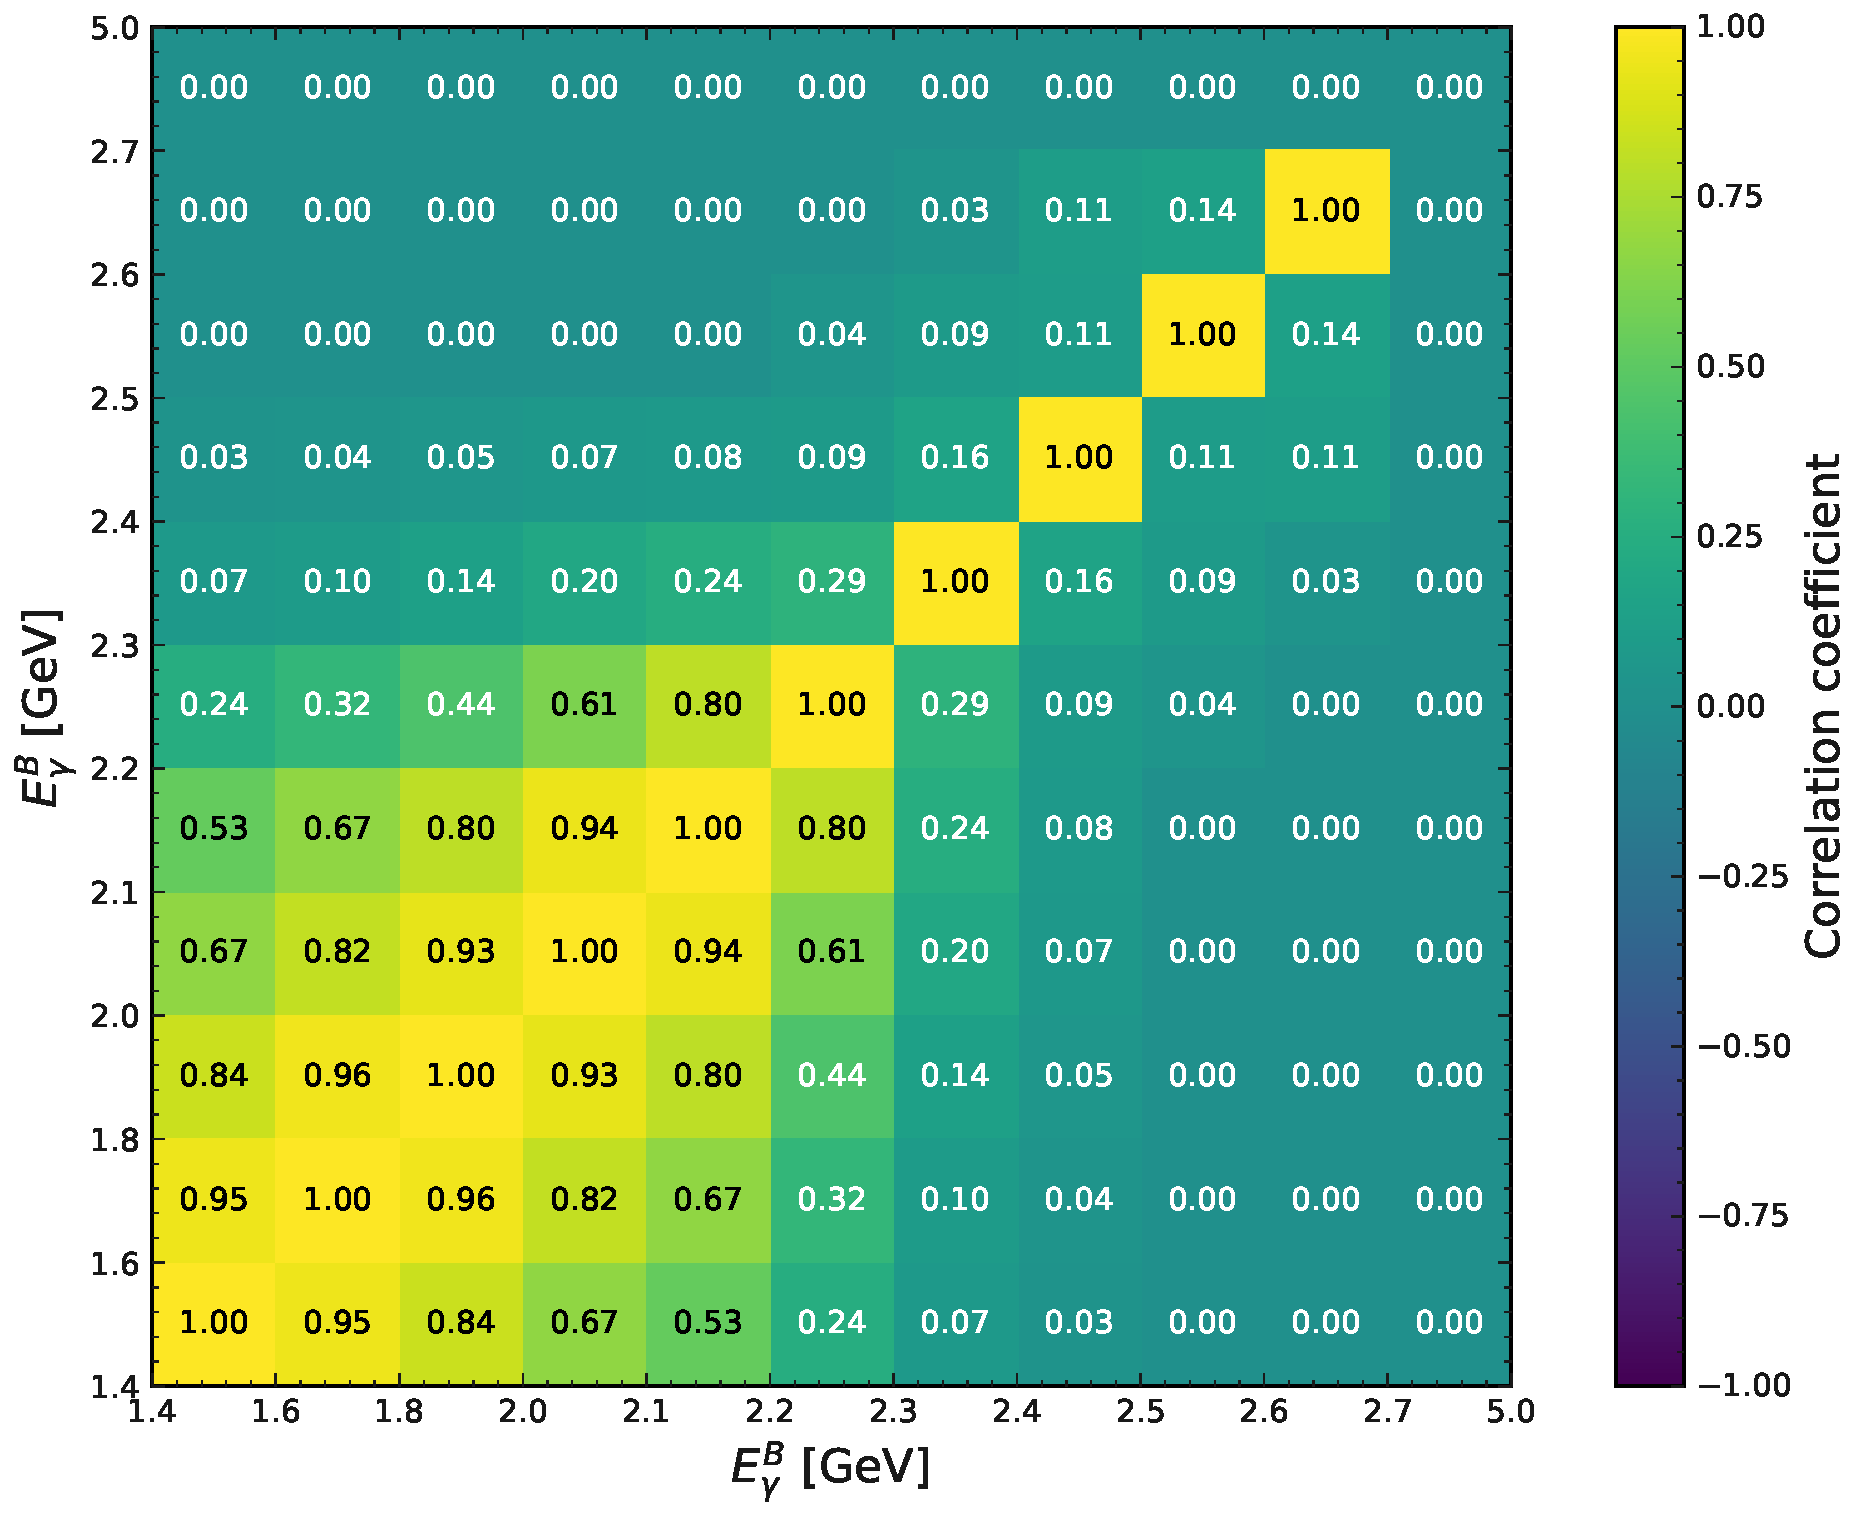
\includegraphics[width=0.5\textwidth]{figures/data_sim_corrections/bbar_correlation_matrix.pdf}
    \caption{\label{fig:bbar_correlation_matrix} The correlation matrix of \BB corrections.
    Particularly low-\EB bins are largely correlated because similar background modes contribute in these regions.
    On the other hand, high-\EB background photons originate more sporadically and from fewer sources, thereby reducing the correlation.
    }
\end{figure}
It can be seen that mostly low-\EB bins are correlated, whereas high-\EB bins show smaller correlations.
Indeed, abundant background processes fall off quickly with increasing \EB.
In the high-\EB region, background photons are rarer and often originate as outliers from a variety of rare decays, decorrelating the bins.

\subsection{Out-of-time photon suppression}\label{sec:out_of_time_photon_suppression}

Although no special corrections are calculated, an additional selection is added to ensure that photons produced by the beam background\footnote{
Particles that are not from the primary collision but are produced by the interactions of the accelerator beam 
and residual gas in the beam pipe or the material of the detector.},
and products of previous collision events are not included in the candidate photon selection.
Such machine-related backgrounds vary based on the experimental conditions and these effects are not well captured by the Belle~II run-period independent simulation that is used in preparation for this analysis.
Therefore, a timing selection requires the photon to be registered in a time window $|\tau_{\gamma}|<200~\ns$ around the collision time.
Furthermore, to reject photons associated with low-quality cluster reconstruction, a $|\tau_{\gamma}|/\Delta\tau_{\gamma}<2$ requirement is added, 
where $\Delta\tau_{\gamma}$ is the uncertainty of the photon timing measurement.
Using a technique analogous to $\epem\ra\mumu$ recoil study, it is observed that it degrades the photon finding efficiency by less than 2\%.
Therefore, these selections are employed with no additional data-to-simulation correction.